\chapter{Applications of Model Comparison}\label{ch:model2}
%!TEX root = main.tex

This chapter presents several applications of the model comparison concepts introduced in Chapter~\ref{ch:model1} (\emph{\nameref{ch:model1}}).

\section{Disease Testing}\label{sec:disease}

Let's imagine there is a rare, one in a million, disease that is lethal but does not have many outward symptoms at first.  A new test boasts 99.9\% accuracy, so you go to get tested, and receive the bad news that you test positive for the disease.  Should you be devastated by the news?  What is the probability that you {\em actually} have the disease?  We are looking at two, quite different, probabilities here.  In the first case, we have the claims of the test which state that {\em if you have the disease, the probability that the test will be positive is 0.999}, or, {\em if you have the disease, test will discover that fact 99.9\% of the time}.  In the second case we have your concern which is, {\em if you test positive for the test, what is the probability that you have the disease}.  In our notation this is:
\beqn
P(\mbox{positive test}|\mbox{disease})&=&0.999\mbox{ (claim from test)}\\
P(\mbox{disease}|\mbox{positive test})&=&?\mbox{ (your concern)}
\eeqn

These two are related by Bayes' Rule (Equation~\ref{eq:bayes}).

The Bayes' Recipe proceeds as follows
\be
\i Specify the prior probabilities for the models being considered

The models we have are simply ``have the disease'' and ``don't have the disease''.  The prior probabilities for these two come from the prevalence of the disease in the population, before you get tested.  Since this is a ``one in a million'' disease, we have

\beqn
\P{disease} &=& \frac{1}{1,000,000}\\
\P{no disease} &=& \frac{999,999}{1,000,000}
\eeqn

\i Write the top of Bayes' Rule for all models being considered

The top of Bayes' Rule comes down to, given the truth of the model (i.e. either with or without the disease), what is the probability of getting the data (i.e. the positive or negative test result).  This is measured by how good the test is. \marginnote{In many medical applications, the false positive rate ($\Pg{positive test}{no disease}$) is not always equal to the false negative rate ($\Pg{negative test}{disease}$), so to say that a test is 99.9\% accurate is actually incomplete - one needs to specify both rates of effectiveness.  In this case, we are assuming that they are the same.}

\beqn
\Pg{positive test}{disease} &=& 0.999
\eeqn
and
\beqn
\Pg{positive test}{no disease} &=& 0.001
\eeqn

So the top of Bayes' Rule looks for both models looks like:

\beqn
\Pg{disease}{positive test} &\sim& \Pg{positive test}{disease} \times \P{disease} \\
&\sim& 0.999 \times \frac{1}{1,000,000}=9.99\E{-7}\\
\Pg{no disease}{positive test} &\sim& \Pg{positive test}{no disease} \times \P{no disease} \\
&\sim& 0.001 \times \frac{999,999}{1,000,000}=9.99\E{-4}
\eeqn

\i Add these values for all models

\beqn
K=9.99\E{-7} + 9.99\E{-4} = 0.000999999
\eeqn

\i Divide each of the values by this sum, $K$, to get the final probabilities

\beqn
\Pg{disease}{positive test} &=& \frac{9.99\E{-7}}{0.000999999} = 0.1\%\\
\Pg{no disease}{positive test} &=& 99.9\%
\eeqn
\ee

Which means that, \emph{overwhelmingly}, if you have a rare one-in-a-million disease, you are very unlikely to have it \emph{even given a 99.9\% accurate positive test for it}!  This is a seriously unintuitive result, so it is helpful to visualize it in another way to build your intuition.

One way to see this result is to visualize it, as in Figure~\ref{fig:disease}.  Here, the numbers are a bit smaller - the disease is 1 out of 200 in a population of 3000, and the test is 99\% accurate.  This means about 15 sick people and about 2985 healthy people.  If all of the sick people test positive, and 1\% of the healthy people test positive due to the 99\% accuracy, we would have 15 sick and 29 healthy people who all test positive.  Even in this case, with much smaller numbers, we see that getting a positive test alone does not imply that it is likely you have the disease.  It depends on the rarity of the disease (the more rare, the less likely) and the false positive rate (the number of healthy people who test positive anyway).  This will vary depending on the disease and the test, but can lead to this unintuitive result, and thus can lead one to make poor medical decisions.

\begin{figure*}
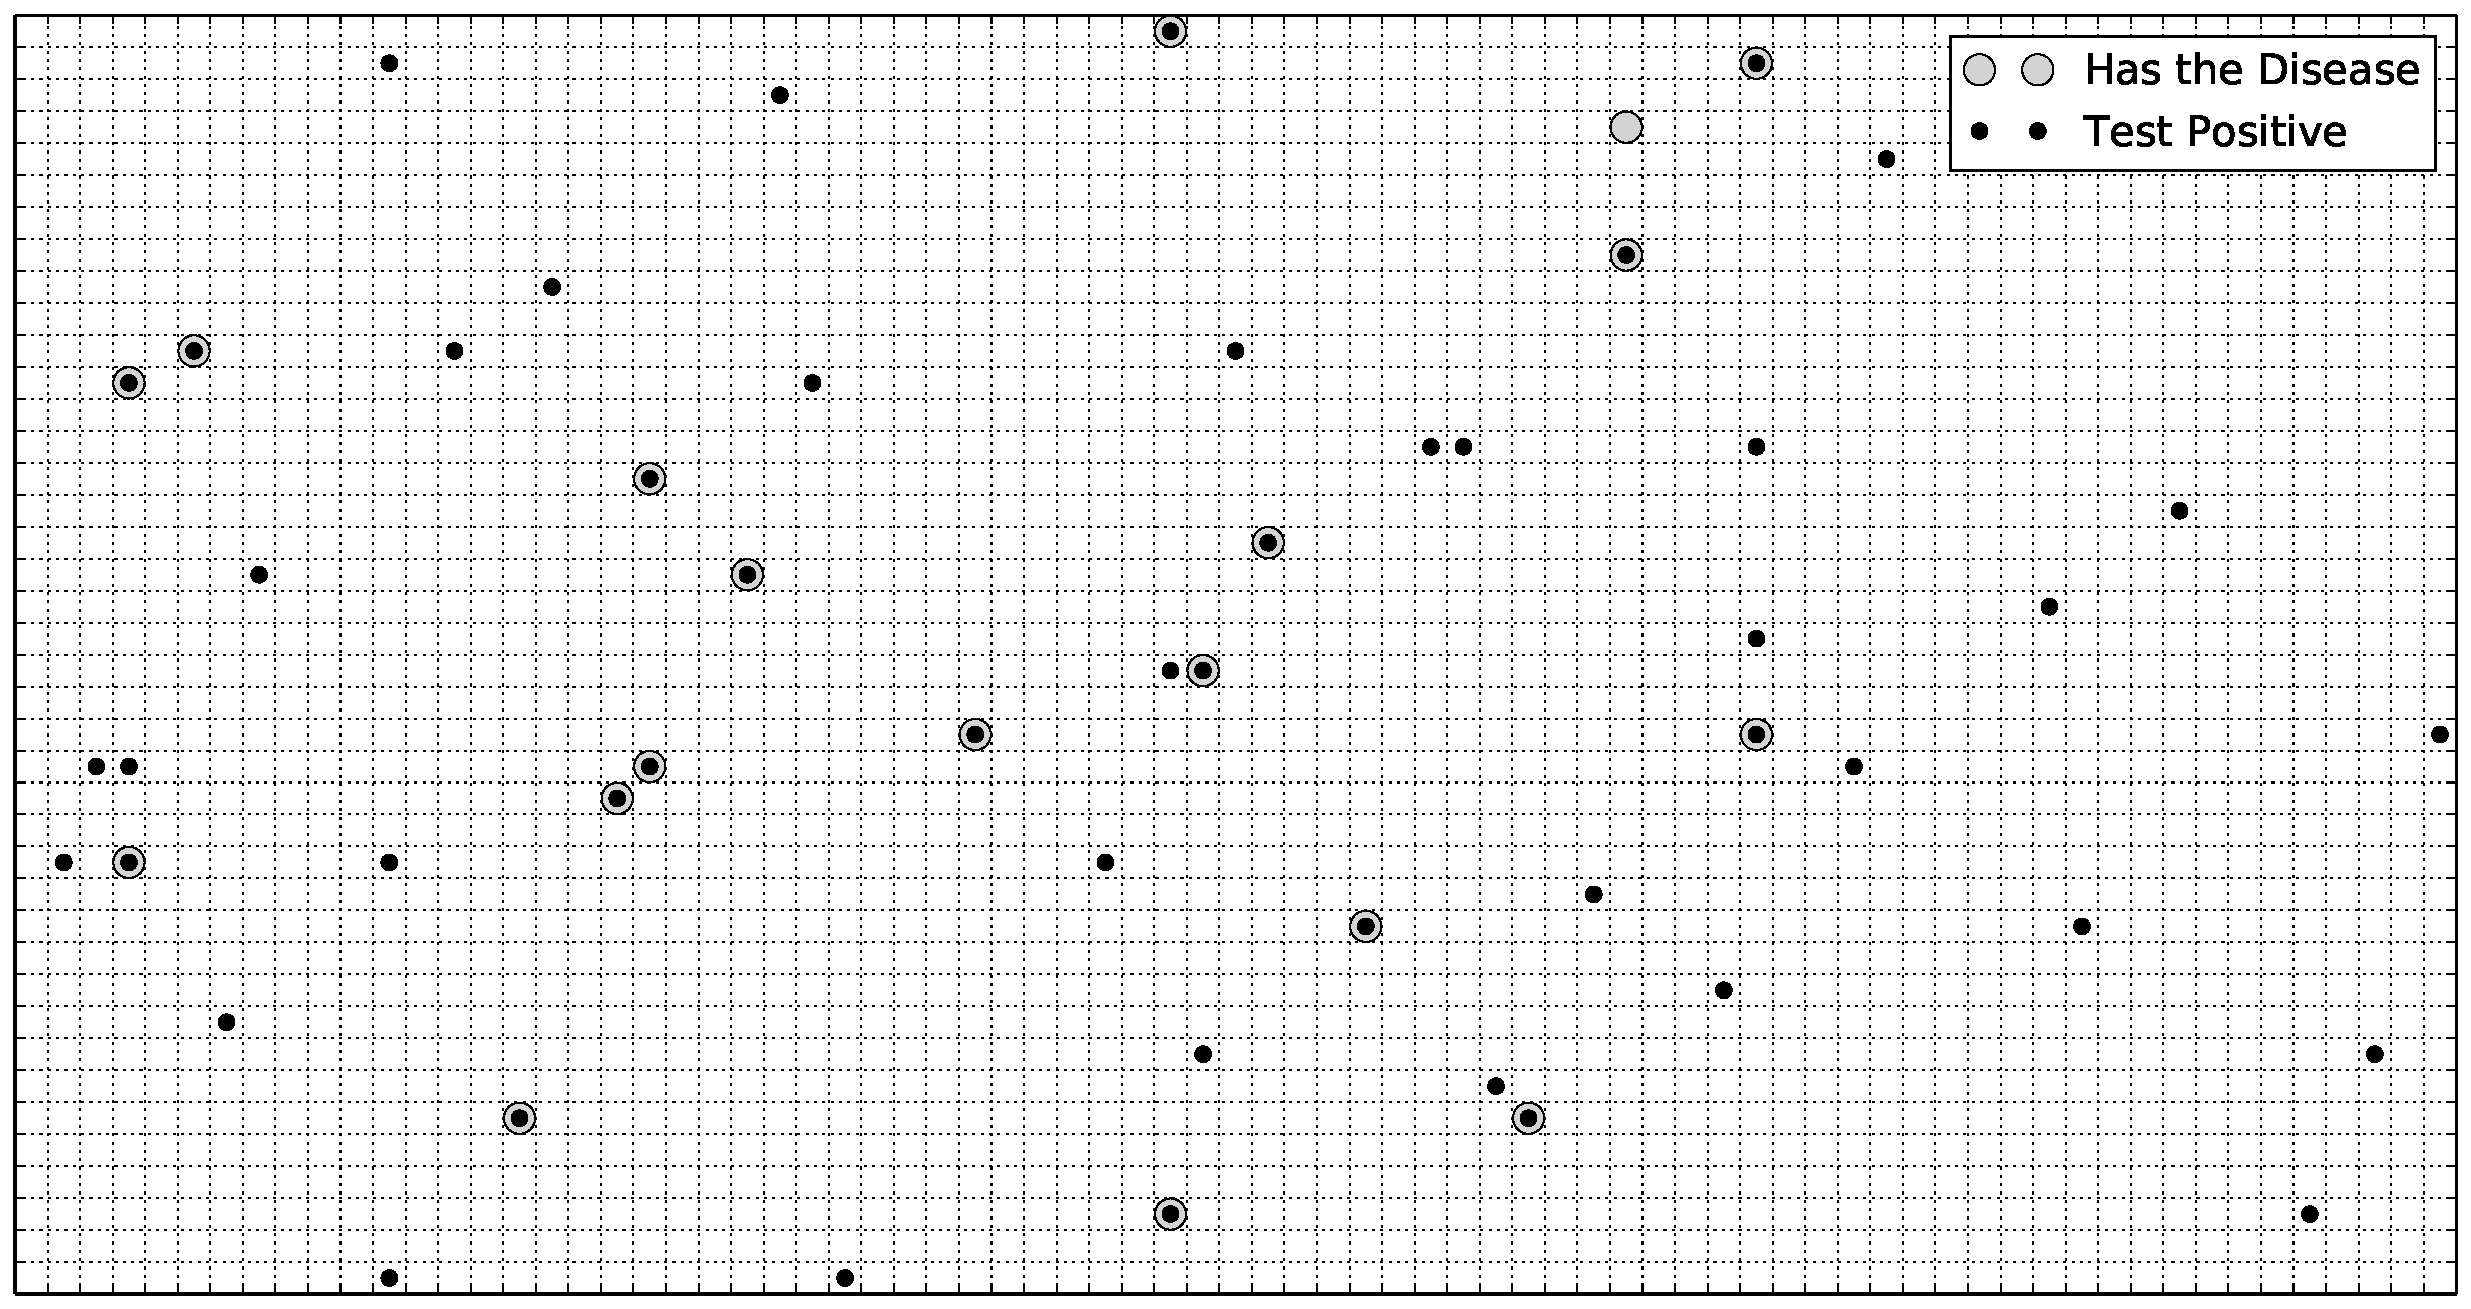
\includegraphics{disease_plot}
\caption{Rare disease and testing.  Shown is a population of 3000 where 1 in every 200 people have the disease (large circles).  A test which is 99\% effective is applied to everyone in the population, and the positive test results (i.e. the test says that you have the disease) are shown ask small black dots. Notice that although nearly all of those that have the disease test positive (a small black dot inside a large circle), there are many false positives (black dot in an empty square) - healthy people that test positive for the disease.  Even though the test is quite good, there are many more healthy people and 1 out of 100 of them will erroneously test positive.}\label{fig:disease}
\end{figure*}

\subsection{Consequences}

This sort of disease testing has serious consequences, especially for rare diseases with tests that aren't precise.  In the book ``The Theory That Would Not Die: How Bayes' Rule Cracked the Enigma Code, Hunted Down Russian Submarines, and Emerged Triumphant from Two Centuries of Controversy'' by Sharon McGrayne there is a discussion concerning the 2009 advice from the U.S. government task force that ``most women in their forties {\em not} to have annual mammograms.'' (emphasis mine)  According to McGrayne,
\begin{quotation}
Thus the probability that a woman who tests positive has breast cancer is only 3\%. She has 97 chances out of 100 to be disease free.
None of this is static. Each time more research data become available, Bayes' rule should be recalculated. As far as Bayes is concerned, universal screening for a disease that affects only 4/10 of 1\% of the population may {\em subject many healthy women to needless worry and to additional treatment which in turn can cause its own medical problems.} In addition, the money spent on universal screening could potentially be used for other worthwhile projects. Thus Bayes highlights the importance of improving breast cancer screening techniques and reducing the number of false positives.\cite{McGrayne:2011fk} (emphasis mine)
\end{quotation}

Thus the proper application of probability theory allows us to separate true but unintuitive things from this which only seem true and intuitive but are in fact false. 

\section{M\&M's}\label{sec:mms}

From various sources I have found the fraction of chocolate M\&Ms candies are red.  The sources found are the following:

\bi
\i Source A: 28\% of M\&Ms are red, 20\% of M\&Ms are orange.
\i Source B: 20\% of M\&Ms are red, 10\% of M\&Ms are orange
\i Source C: 13\% of M\&Ms are red, 21\% of M\&Ms are orange.
\ei

From actually counting of a bag of M\&Ms I found the following data:

\bi
\i 3 red M\&Ms in 17 total ($R=3, N=17$)
\ei

The question is, {\em which source can we trust the most?}  Here we follow Bayes' recipe,

\bi
\i Specify the prior probabilities for the models being considered
\beqn
P(A)=P(B)=P(C)=1/3
\eeqn
\i Write the top of Bayes' Rule (i.e. likelihood $\times$ prior) for all models being considered
\beqn
P(A|R=3, N=17) &\sim& \nchoosek{17}{3} 0.28^{3}(1-0.28)^{17-3}\times \frac{1}{3}\\
P(B|R=3, N=17) &\sim& \nchoosek{17}{3} 0.20^{3}(1-0.20)^{17-3}\times \frac{1}{3}\\
P(C|R=3, N=17) &\sim& \nchoosek{17}{3} 0.13^{3}(1-0.13)^{17-3}\times \frac{1}{3}
\eeqn
\i Add these values for all models, to get $K$
\beqn
P(A|R=3, N=17) &\sim& 0.05006\\
&&+\\
P(B|R=3, N=17) &\sim& 0.07975\\
&&+\\
P(C|R=3, N=17) &\sim& 0.07087 \\ \cline{1-3}
K&=& 0.20068
\eeqn

\i Divide each of the values by this sum, $K$, to get the final probabilities

\beqn
P(A|R=3, N=17) &=& 0.05006/0.20068 = 0.250\\
P(B|R=3, N=17) &=& 0.07975/0.20068 = 0.397\\
P(C|R=3, N=17) &=& 0.07087/0.20068 = 0.353
\eeqn

\ei

So we are most confident in Source B, although none of them really changed by a lot - there is no clear winner.

\subsection{Updating with other data}

\bi
\i 5 orange M\&Ms in 16 total  ($G=5, N=16$)
\ei

Again, we follow the same recipe, starting with out posterior probabilities from above as our starting {\em prior} probabilities - they are {\em prior} to the new data.

\bi
\i Specify the prior probabilities for the models being considered
\beqn
P(A|{\rm old\ data}) &=& 0.250\\
P(B|{\rm old\ data}) &=& 0.07975/0.20068 = 0.397\\
P(C|{\rm old\ data}) &=& 0.07087/0.20068 = 0.353
\eeqn
\i Write the top of Bayes' Rule (i.e. likelihood $\times$ prior) for all models being considered
\beqn
P(A|G=5, N=16 \mbox{ {\bf and} old data}) &\sim& \nchoosek{16}{5} 0.20^{5}(1-0.20)^{16-5}\times 0.250\\
P(B|G=5, N=16 \mbox{ {\bf and} old data}) &\sim& \nchoosek{16}{5} 0.10^{5}(1-0.10)^{16-5}\times 0.397\\
P(C|G=5, N=16 \mbox{ {\bf and} old data}) &\sim& \nchoosek{16}{5} 0.21^{5}(1-0.21)^{16-5}\times 0.353
\eeqn
\i Add these values for all models, to get $K$
\beqn
P(A|{\rm data}) &\sim& 0.0300\\
&&+\\
P(B|{\rm data}) &\sim& 0.00544\\
&&+\\
P(C|{\rm data}) &\sim& 0.0471 \\ \cline{1-3}
K&=& 0.08254
\eeqn

\i Divide each of the values by this sum, $K$, to get the final probabilities

\beqn
P(A|{\rm data}) &=& 0.0300/0.08254 = 0.363\\
P(B|{\rm data}) &\sim& 0.00544/0.08254 = 0.0659\\
P(C|{\rm data}) &\sim& 0.0471/0.08254 = 0.5706
\eeqn

\ei

Given this new data, we update our state of knowledge, and we're much more confident that Source C is the best one.  It is clear that Source B is unlikely, with a probability of only about 6.5\%.  We could extend this example with more data, and more models if we'd like.



\section{Psychic Octopi}

There was a German octopus named Paul\cite{wiki:psychic_octopus} who was claimed to be psychic during his lifetime.  He was given this designation because he was supposedly able to pick the result of World Cup matches before they occurred\footnote{The basic procedure for Paul to make a ``prediction'' was for his trainers to present two food dishes, labeled with a flag representing the two countries, respectively, competing.  Whichever food dish Paul chose first was his prediction for the winner of the game.}.  His impressive results, across 2 years, shown in Figure~\ref{fig:paul} can be summarized as follows:

\beqn
{\rm data}&\equiv& \mbox{12 out of 14 correctly predicted}
\eeqn


\begin{figure}
\begin{tabular}{|c|}\hline
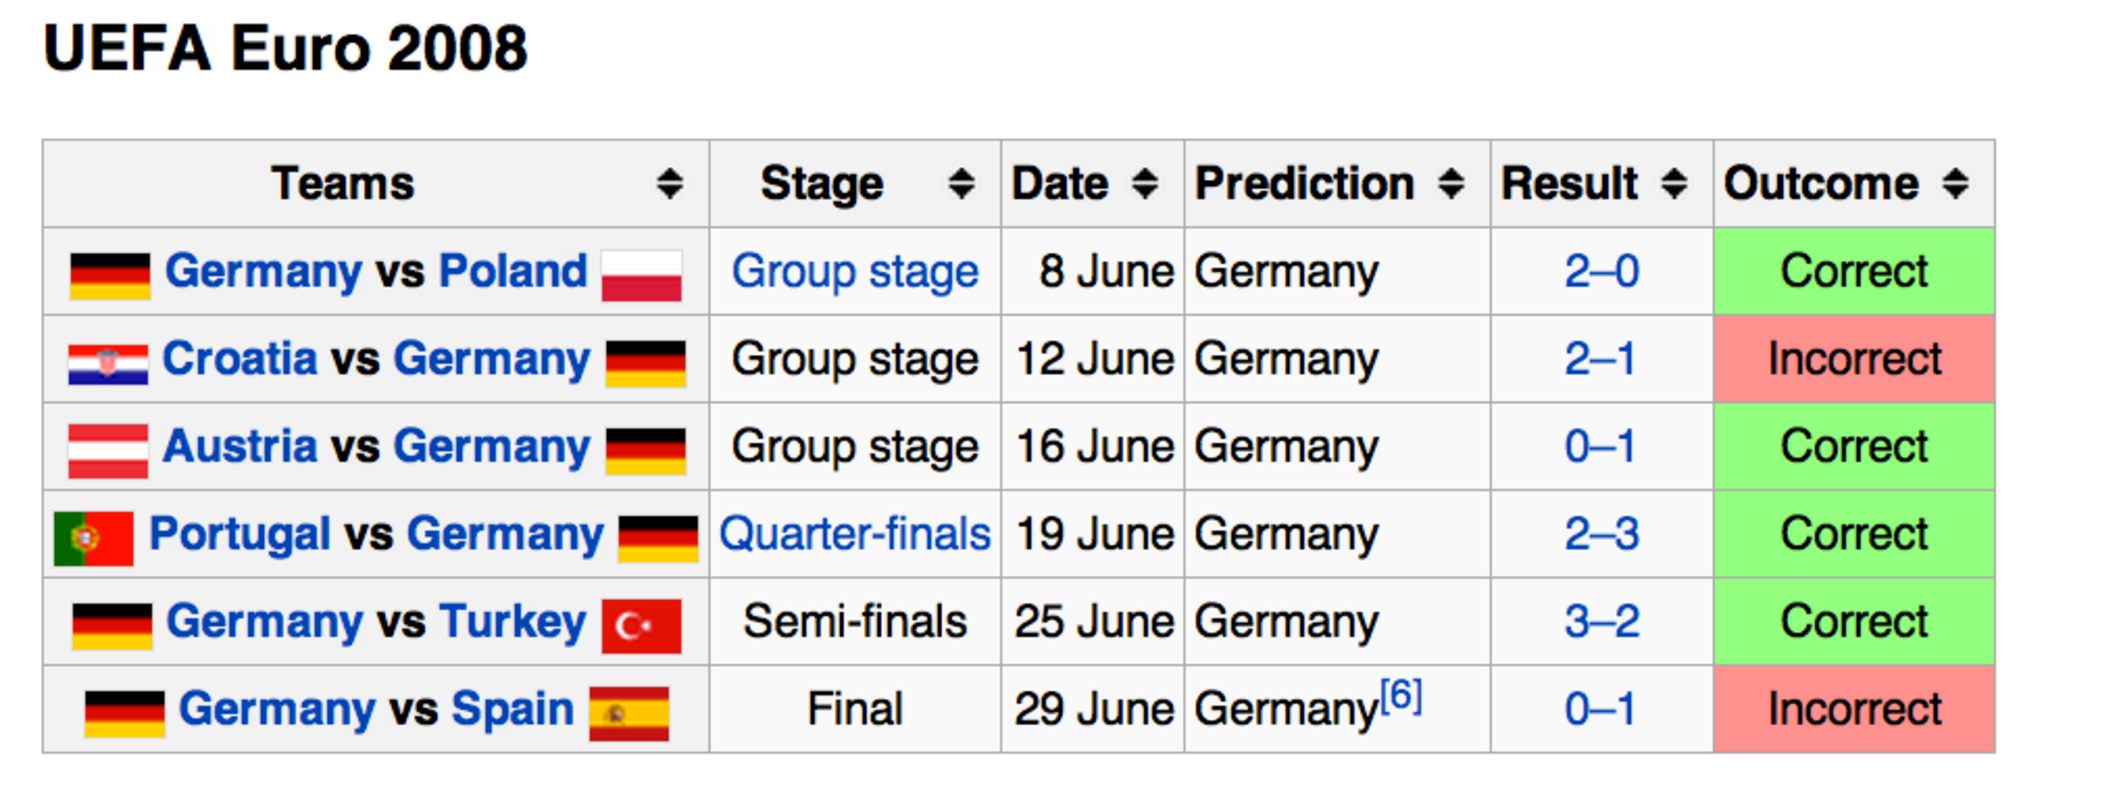
\includegraphics{paul1}\\
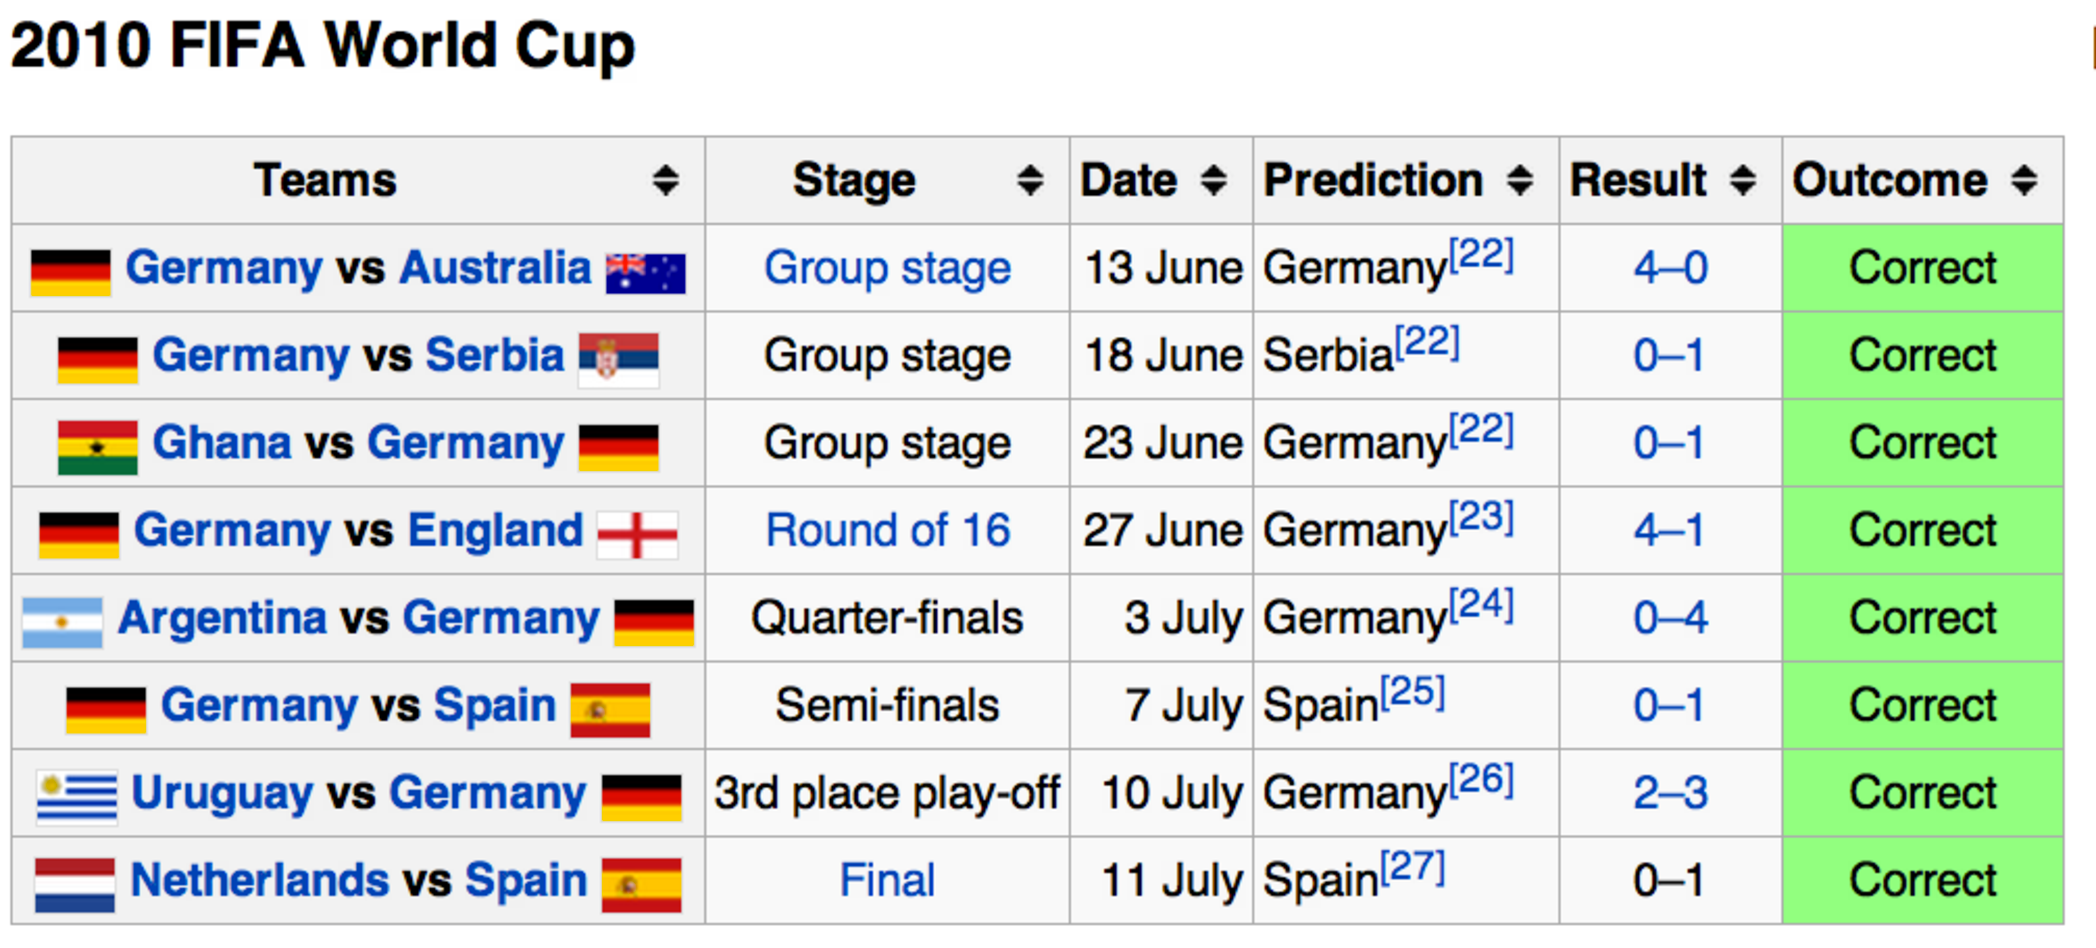
\includegraphics{paul2}\\ \hline
\end{tabular}
\caption{The full results of the predictions of Paul the Octopus, reproduced from \href{http://en.wikipedia.org/wiki/Psychic_octopus}{en.wikipedia.org/wiki/Psychic\_octopus}.}
\label{fig:paul}
\end{figure}

The question we have to ask is, is this data strong evidence for a psychic octopus?  In order to have a well-posed problem we need the following three components:

\be
\i a set of hypotheses, or models, to compare - we need at least two, otherwise the question is meaningless
\i for each model, an equation denoting the {\em likelihood}, or in other words, how probable is the data given the particular model
\i a specification of the {\em prior} probability, or in other words, how likely was our model before we saw the data
\ee

\subsection{Making a Well Posed Problem}

We are interested in the probability of this octopus being psychic, given this data, or
\beqn
P({\rm psychic}|{\rm data})
\eeqn 
which really is an example of a model comparison, or hypothesis testing.  In any kind of model comparison, we need to have {\em multiple models} to compare to in order to proceed.  The models we consider constrain the problem, and define which ideas we are willing to consider.  To be specific, as a first step, let's consider the following two models
\beqn
H&:=&\{\mbox{Paul is psychic}\} \\
R&:=&\{\mbox{Paul is completely random, like a coin flip}\}
\eeqn

The next step is to be able to assign probabilities from these models.  It is easy for the {\em random} hypothesis
\beqn
P(\mbox{correct prediction}|R) &=& 0.5 \\
P(\mbox{incorrect prediction}|R) &=& 0.5
\eeqn

What does it mean to be psychic?  What is the probability of getting a correct result if you are psychic?  According to James Randi\cite{randi1982flim} many of the psychics and dowsers claim 100\% accuracy in their predictions before they are tested.  However this would mean a {\em single} wrong answer would drive the probability of that model to {\em zero}: a perfect predictor cannot, logically, make any mistakes.  For our case here, we choose to be generous to the psychic and allow for a reasonable failure rate, using 90\% as our accuracy, thus
\beqn
P(\mbox{correct prediction}|H) &=& 0.9 \\
P(\mbox{incorrect prediction}|H) &=& 0.1
\eeqn

Specifying the prior probability of these two models is a bit more challenging.  It seems reasonable to assign a small prior probability to a psychic octopus - how many psychic octopi have you ever encountered?  A small, but still quite conservative value, would be 1/100, so we have for the two models\marginnote{It is possible that we could be accused of an anti-psychic bias here, especially from someone who is a true believer.  Why shouldn't the prior be $P(H)=1/2$?  If you had no world experience, that is what you'd start with, but then the behavior of the first octopi that you encounter would generally lower your assignment of the probability of the next octopi being psychic.  After enough world experience, updating your probability with Bayes' Rule, you'd arrive at a very small prior for Paul, the current octopus we are examining.}:
\beqn
P(H)&=& 1/100 \\
P(R)&=& 99/100
\eeqn

\subsection{The First Model Comparison}
Now that we've set up the problem, we can apply the Bayes' Recipe
\be
\i Specify the prior probabilities for the models being considered
\beqn
P(H) &=& 1/100 \\
P(R) &=& 99/100
\eeqn
\i Write the top of Bayes' Rule for all models being considered
\beqn
P(H|{\rm data}=\mbox{12 out of 14})&\sim& P({\rm data}=\mbox{12 out of 14}|H)P(H) \\
P(R|{\rm data}=\mbox{12 out of 14})&\sim& P({\rm data}=\mbox{12 out of 14}|R)P(R) 
\eeqn
where we are using the symbol $\sim$ to denote {\em proportionality} or {\em related to}.  Essentially, by calculating the top of Bayes' Rule first, the numbers are not {\em equal} to the final (i.e. posterior) probabilities but must be rescaled to make sure that they add up to 1.  This is done in the final step.  Up until that rescaling, we use the symbol $\sim$ and think of it as {\em related to}.
\i Put in the likelihood and prior values
\beqn
P(H|{\rm data}=\mbox{12 out of 14})&\sim& \nchoosek{14}{12}0.9^{12}0.1^{14-12}\times \frac{1}{100} \\
&=&0.00257\\
P(R|{\rm data}=\mbox{12 out of 14})&\sim& \nchoosek{14}{12}0.5^{12}0.5^{14-12}\times \frac{99}{100}\\
&=&0.00549\\
\eeqn
\i Add these values for all models
\beqn
K=0.00257+0.00549= 0.00806
\eeqn
\i Divide each of the values by this sum, $K$, to get the final probabilities
\beqn
P(H|{\rm data})=\frac{0.00257}{0.00806}=0.32\\
P(R|{\rm data})=\frac{0.00549}{0.00806}=0.68
\eeqn
\ee
and the psychic loses!  We continue this problem discussing the potential {\em anti-psychic} bias in the presentation of the problem.  

\subsection{Furthering the Comparison}

Typically, a person who is supportive of psychic phenomena would choose a prior for our psychic hypothesis ($H$) that would be at least as large as the prior for the random hypothesis ($R$).  In this case, the (posterior) probability of the octopus being psychic given the data of 12 correct out of 14 would be much higher.  After ``ruling out'' the random octopus hypothesis, we'd be left with psychic.  But is that all that is really left?  No, and the analysis is easy to do.  

Once presented with the success of Paul, most people instantly are suspicious of random octopus, but don't adopt psychic octopus as the answer.  Perhaps the keepers, being German, biased the data taking a little bit.  Perhaps the octopus chose flags with bright yellow stripes.  Notice that each of these cases still results in  similar data - the octopus would have gotten 11 or 12 out of 14, but the \emph{prior} probability of these cases should be much higher than psychic, even if lower than random.  We leave it as an exercise to perform the calculation in this case, but it is directly parallel to the \emph{Nines} deck example of Section~\ref{sec:multiplehypotheses} on page~\pageref{sec:multiplehypotheses}.




\section{Monty Hall Problem}\label{sec:monty_models}

This problem was introduced in Section~\ref{sec:monty}. 

\example{Is it better to switch doors? - Monty Hall Problem revisited}

 You may recall that we were presented with a choice of 3 doors where a car is behind one and goats behind the others. Having picked one, the host opens up a door with a goat, and offers you the opportunity to change your answer.  In order to assess the probabilities, we must remember that 
\be
\i the host {\em never} opens your door
\i the host {\em always} opens a door with a goat
\ee

We'll go through a specific example, that of you choosing door 1 and the host opening door 2.  The analysis proceeds in identical ways for the other possibilities.  We apply the Bayes' Recipe, where the models under consideration are 

\bi
\i ``car behind door 1''
\i ``car behind door 2''
\i ``car behind door 3''
\ei

The Bayes' Recipe proceeds as follows
\be
\i Specify the prior probabilities for the models being considered
\beqn
\Pg{car 1}{you 1} &=& 0.333 \\
\Pg{car 2}{you 1} &=& 0.333 \\
\Pg{car 3}{you 1} &=& 0.333
\eeqn
where, for example, $\Pg{car 1}{you 1}$ represents the probability that the door contains the car given that you chose door 1.  Since your choice of door doesn't add any information about the location of the car, all of the probabilities are equal.

\i Write the top of Bayes' Rule for all models being considered
\beqn
\Pg{car 1}{you 1, host 2} &\sim& \Pg{host 2}{you 1, car 1}\Pg{car 1}{you 1} \\
\Pg{car 2}{you 1, host 2} &\sim& \Pg{host 2}{you 1, car 2}\Pg{car 2}{you 1} \\
\Pg{car 3}{you 1, host 2} &\sim& \Pg{host 2}{you 1, car 3}\Pg{car 3}{you 1}
\eeqn
\i Put in the likelihood and prior values

Due the restrictions on the host above, the host cannot open a door with a car, so $\Pg{host 2}{you 1, car 2}=0$.  In the case where you choose door 1 and the car is also behind door, the host has the freedom to choose either door 2 or door 3, so $\Pg{host 2}{you 1, car 1}=0.5$.  Where the information comes in is when the car is behind door 3 and you've chosen door 1.  In that case, the host cannot open your door (door 1) or the door with the car (door 3) and {\em must} open door 2.  Thus, $\Pg{host 2}{you 1, car 3}=1$.  

The final result of this step is
\beqn
\Pg{car 1}{you 1, host 2} &\sim& 0.5 \cdot 0.333\\
\Pg{car 2}{you 1, host 2} &\sim& 0 \cdot 0.333 \\
\Pg{car 3}{you 1, host 2} &\sim& 1 \cdot 0.333
\eeqn

\i Add these values for all models
\beqn
K=0.5 \cdot 0.333+ 1 \cdot 0.333 = 0.5
\eeqn
\i Divide each of the values by this sum, $K$, to get the final probabilities
\beqn
\Pg{car 1}{you 1, host 2} &=& \frac{0.5 \cdot 0.333}{0.5}=0.333\\
\Pg{car 2}{you 1, host 2} &=& \frac{0 \cdot 0.333}{0.5}= 0 \\
\Pg{car 3}{you 1, host 2} &=& \frac{1 \cdot 0.333}{0.5}= 0.666
\eeqn
\ee

Thus, in the case, given that you choose door 1 and the host chooses 2, the probability that the car is behind door 1 (your door) is 0.333 and the other door (door 3) is 0.666.  Following the same steps through the other cases, we get in summary
\begin{center}
\begin{tabular}{ccccc}
& & \multicolumn{3}{|c|}{Probability of...} \\
Your Choice & Host Choice & Car Behind 1 & Car Behind 2 & Car Behind 3 \\\hline
1 & 1 & \multicolumn{3}{c}{\emph{(host can't open your door)}} \\
1 & 2 & 0.333 & 0 & 0.666 \\
1 & 3 & 0.333  & 0.666 & 0\\\hline
2 & 1 &  0 &0.333 & 0.666 \\
2 & 2 & \multicolumn{3}{c}{\emph{(host can't open your door)}} \\
2 & 3 &   0.666 & 0.333 & 0  \\\hline
3 & 1 & 0 & 0.666 & 0.333 \\
3 & 2  & 0.666 & 0 & 0.333\\
3 & 3 & \multicolumn{3}{c}{\emph{(host can't open your door)}}
\end{tabular}
\end{center}

In summary, it is \emph{always} better to switch to the remaining door, given these rules.
